\section{Results}
\label{SECIV}\label{sec:results}

In this section we test our implementation of the \lloid\ method using the
pipeline described in the previous section.  We calculate the measured \SNR\
loss due to the approximations of the \lloid\ method and our implementation of
it.
%We answer the following questions:
%
%I) What is the measured loss of \SNR\ due to the approximations used in the
%\lloid\ algorithm in a realistic analysis pipeline?
%
%II) What is the measured latency of the implementation described in section
%\ref{sec:implementation}?
%
%III) What is the measured computational cost of the implementation described in
%section \ref{sec:implementation}?


\subsection{Measured \SNR\ loss}

We expect two known contributions to the \SNR\ loss to arise in our
implementation of the \lloid\ algorithm.  The first is the \SNR\ loss due to
the truncation of the \SVD\ basis, which is fundamental, and estimates for it
exist~\cite{Cannon:2010p10398}.  The second comes from non ideal
implementations of resampling that cause signal loss.  We have measured the
effect of the resampling in the pipeline alone on a single waveform to gauge
the magnitude of the loss.  It is shown in figure \ref{fig:hist-interpolate} as a
function of the quality of the {\tt audioresample} element (which is
proportional to the filter length used).  In both cases we have to compare the
\SNR\ loss to the expected \SNR\ loss that arises from the discreteness of the
template bank which is typically $\sim 3\%$.  We will consider a comparable
\SNR\ loss to be tolerable, but ideally would like to have a factor of 10 lower
loss from the \lloid\ implementation (i.e. no more than $\sim 0.3 \%$).

It is also within reason that some \SNR loss could arise from other suboptimal
implementations of the \lloid\ algorithm in our test pipeline.  To gauge
accurately how well the pipeline is performing we tested the response to a
delta function.  This produces time reversed versions of the original template
waveforms. By taking the inner product of the impulse response for each channel
with the time reversed template, we can gauge very accurately the loss in
expected \SNR\ due to the approximations we have made and any inadequacies in
our implementation. 

\subsubsection{Checking the effect of the \SVD\ tolerance}

In this section we check the effect of the \SVD\ tolerance parameter defined in
~\cite{Cannon:2010p10398}.  By changing the tolerance of the reconstruction of
the physical waveforms one effects directly the mismatch that results from the
truncation of the orthogonal filter matrix.  The conditions presented here are
more complicated than in the original work~\cite{Cannon:2010p10398} due to the
inclusion of the time sliced templates and resampling.  \FIXME{However, we find
that the results are quite as expected.}  Figure \ref{fig:hist-svd-tolerance}
demonstrates that it is possible to acheive typical \SNR\ losses of $\ll1\%$.
However, we do notice that the mismatch saturates with respect to the tolerance.
This could be the effect of the resampling, or another \SNR\ loss that we did
not model or expect.  However the saturation is still an order of magnitude below our target mismatch of $\sim 0.3 \%$.  We find that an \SVD\ tolerance of
$\left(1-10^{-4}\right)$ is adequate. 
%
\begin{figure}
	\begin{center}
		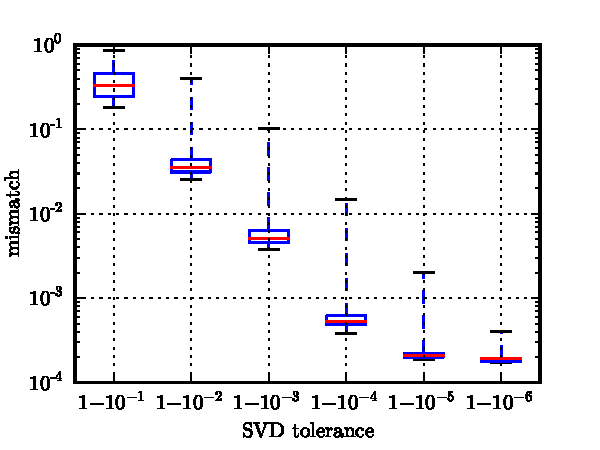
\includegraphics{bw.pdf}
		\caption{\label{fig:hist-svd-tolerance}
Box-and-whisker plot of mismatch between nominal
template bank and \lloid\ measured impulse respones.  The \textsc{svd}
tolerance is varied from $\left(1-10^{-1}\right)$ to $\left(1-10^{-6}\right)$.
The diminishing improvement is caused by some other limitation in the pipeline.}
	\end{center}
\end{figure}

\subsubsection{Checking the effect of the interpolation filter length}

Next, keeping the \SVD\ tolerance fixed at $\left(1-10^{-6}\right)$, we checked the
impact of changing the filter length used to interpolate the decimated data
back up to the full sample rate.  The results are in figure
\ref{fig:hist-interpolate}.  We find that a filter length of 16 is sufficient
to produce mismatches at our target of $\sim 0.3 \%$.
%
\begin{figure}
	\begin{center}
		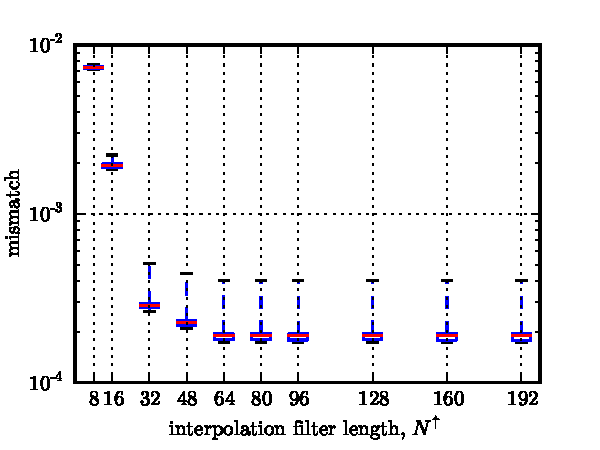
\includegraphics{bw_resample.pdf}
		\caption{\label{fig:hist-interpolate} Box-and-whisker plot of
mismatch between nominal template bank and \lloid\ measured impulse respones.
The length $N^\uparrow$ of the interpolation filter is varied from 8 to 192.
The \textsc{svd} tolerance is kept fixed at $(1-10^{-6})$.  The lines in the
center of the boxes denote the medians.  The upper and lower boundaries of the
boxes show the upper and lower quartiles.  The whiskers denote the minimum and
maximum mismatch over all templates.}
	\end{center}
\end{figure}



%\subsection{Measured latency}

%In order to check the latency of our implementation of the \lloid\ algorithm we
%used the pipeline described in \ref{fig:pipeline} with a live source connected
%to the input.  We then measured the timestamp of the live source and the output
%of the final \SNR\ time series.  Since \gstreamer\ is not a
%sample-in-sample-out realtime infrastructure, it does work by passing small
%buffers of data and filtered data through the pipeline.  We set the buffer size
%on the input to be 1/4 s.  In an ideal case the latency should be nearly 1/4 s.
%However, it is necessary to queue things in the pipeline to assure that there
%are no issues with threading. Sometimes buffers get delayed.  We measured the
%average filtering latency to be \FIXME{1 s}.

%\subsection{Measured computational cost}

%Using the pipeline described previously, we also measured the computational
%cost.  We used an 8 socket, quad core AMD\texttrademark\ machine operating at
%2.7 GHz per core.  We found that filtering \FIXME{657} templates in real time
%required about \FIXME{6} of the available cores.  We thus conclude that we
%require about 1 core for every \FIXME{100} templates.  We note that this is
%well within the computational limits of a modern, computing cluster assuming
%that the scaling holds for the entire mass range of interest, we would need
%about \FIXME{300} cores per detector.  This requirment should be even less of a
%burden in the advanced detecor era, when presumably clusters built in that era
%will have a factor of 4 or 8 more cores than the ones today. 

